\documentclass[a4paper]{jsarticle}
\usepackage[dvipdfmx]{graphicx}
\usepackage{../math_note, exercise}
\renewcommand{\thesection}{Ex2.\arabic{section}}

\newcommand{\shO}{\mathcal{O}}
\newcommand{\Sch}{\mathbf{Sch}}
\newcommand{\Var}{\mathbf{Var}}
\newcommand{\Rings}{\mathbf{Rings}}
\newcommand{\red}[1]{#1_{\text{red}}}
\newcommand{\basesp}{\operatorname{sp}}
\newcommand{\CoverU}{\mathfrak{U}}
\newcommand{\OpenIn}{\text{ :: open in }}
\newcommand{\ClosedIn}{\text{ :: open in }}

\begin{document}

\section{$(D(f), \shO_X|_{D(f)}) \homeo (\Spec A_f, \shO_{\Spec A_f})$} %% Ex2.1 
    $A$ :: ring, $X=\Spec A$, $f \in A$とし,$D(f)=(V((f)))^c$とする.
    $S=\{1,f,f^2,\dots\}$とし,以下のように写像を定める.
    \begin{defmap}
        \phi:& D(f)& \to& \Spec A_f \\ 
        {}& \I{p}& \mapsto& S^{-1}\I{p} \\
        {}& \I{q} \cap A& \mapedfrom& \I{q}
    \end{defmap}
    $\I{p}$は$S$と共通部分を持たない素イデアルだから,
    Ati-Mac Prop3.11より,$\phi$は全単射.

    $C \ClosedIn D(f)$とする.
    この時,
    \[ C=\{ \I{p} \in \Spec A ~|~ \I{I} \subseteq \I{p}, (f) \not \subseteq \I{p} \} \]
    となるイデアル$\I{I} \subset A$が存在する.
    Ati-Mac Prop3.3より,$\phi$は単射を保つから,$\phi(C)$もclosed.
    逆に$D \ClosedIn \Spec A_f$をとる.
    再びAti-Mac Prop3.11より,$\Spec A_f$の任意の元は拡大イデアルだから,
    \[ D=\{ \phi(\I{p}') \in \Spec A_f ~|~ \phi(\I{I}') \subseteq \phi(\I{p}'), \phi(f) \not \subseteq \phi(\I{p}') \} \]
    と書ける.
    つまり,$D=\phi(V(\I{I'}))$.
    $\phi$は全単射なので$\phi^{-1}(D)=V(\I{I'})$となり,これはclosed.
    以上より$\phi$が同相写像であることがわかった.

    Prop2.3と同様にlocally ringed spaceの射を構成しておく.
    これは
    \[ f: \I{p} \mapsto \phi^{-1}(\I{p}),~~ f^{\#}: \shO_{\Spec A_f}(-) \mapsto \shO_X|_{D(f)}(\phi(-)) \]
    で定義される.

\section{IF $X$ :: scheme, and $U \OpenIn X$, then $(U,\shO_X|_U)$ :: scheme.} %% Ex2.2 
    $X$はschemeだから,開被覆$\{U_{\lambda}\}_{\lambda \in \Lambda}$が存在し,
    $(U_{\lambda}, \shO_X|_{U_{\lambda}})$はaffine schemeとなる.
    すなわち,
    $R_{\lambda}$ :: ringが存在して
    \[ (U_{\lambda}, \shO_X|_{U_{\lambda}}) \homeo (\Spec R_{\lambda}, \shO_{\Spec R_{\lambda}}) \]
    と書ける.

    $V_{\lambda}=U \cap U_{\lambda}$とすると,$\{V_{\lambda}\}$は$U$の開被覆である.
    そして各$V_{\lambda} \subseteq U_{\lambda}$はaffine schemeの開集合.
    教科書pp.70-71から,affine schemeのopen baseは
    $D(f)~(f \in R_{\lambda})$の形の開集合全体である.
    したがって,各$V_{\lambda}$について,
    以下のような条件を満たす$R_{\lambda}$の部分集合$F_{\lambda}$が取れる.
    \[ V_{\lambda}=\bigcup_{f \in F_{\lambda}} D(f). \]
    まとめると,
    \[ U=\bigcup_{\lambda \in \Lambda} V_{\lambda}=\bigcup_{\lambda \in \Lambda} \bigcup_{f \in F_{\lambda}} D(f). \]
    $f \in R_{\lambda}$であるとき,
    $D(f) \subseteq U_{\lambda}=\Spec R_{\lambda}$とEx2.1より$(D(f), \shO_{U_{\lambda}}|_{D(f)})$はaffine.
    よって$U$はaffine schemeで被覆される.
    ($\shO_U:=\shO_X|_U$に注意.)

\section{Reduced Schemes.} %% Ex2.3 
    scheme $(X, \shO_X)$がreducedとは,
    任意の開集合$U \subseteq X$について$\shO_X(U)$がベキ零元を持たない,
    すなわち$\shO_X(U)$がreduced ringである,ということ.
    $(X, \shO_X)$のreduced scheme $(X, \red{(\shO_X)})$を,
    presheaf $U \mapsto \shO_X(U)/\Nil(\shO_X(U))$のsheafificationとする.
    この$X$から得られたreduced schemeを$\red{X}$と書く.

    \subsection{$(X, \shO_X)$ :: reduced $\iff$ $\Forall{P \in X} \shO_{X,P}$ :: reduced.}
    両者の対偶を示す.
    \paragraph{$(\impliedby)$}
    $U \OpenIn X, s \in \shO_X(U), s \neq 0$とする.
    $s$がnilpotentであったと仮定すると,$s^n=0$となる$n \in \N$が存在する.
    $s \neq 0$から,ある点$P \in U$においては$s(P) \neq 0$.
    しかし$s^n(P)=0=(s(P))^n$なので,$s(P) \in \shO_{X, P}$はnilpotent.

    \paragraph{$(\implies)$.}
    ある点$P$において,$a/f \in \shO_{X,P} \cong A_{\I{p}_P}$がnilpotentであったとする.
    この時,$P$の開近傍$D(f)$上で定義される定値写像$c(*)=a/f$が取れる.
    明らかにこの写像は$\shO_X(D(f))$の元で,しかもnilpotent.

    \subsection{$(X, \red{(\shO_X)})$ :: scheme.}
    $(X, \shO_X)$がaffine schemeだと仮定して証明する.
    調べる必要があるのは,$\red{(\shO_X)}$はsheaf of ring on $\Spec A$であること,
    すなわち以下が成り立つことである.
    \[
        \Forall{U \OpenIn X} \Forall{s \in \red{(\shO_X)}(U)}
        \Forall{\I{P} \in X} P \in {}^{\exists} V \subseteq U \Forall{\I{q} \in V}
        s(Q) \in A_{\I{q}}.
    \]
    $s \in \red{(\shO_X)}(U)$を任意に取る.
    sheafificationのやり方から,点$P$の十分小さな開近傍$V$について
    $s \in \shO_X(U)/\Nil(\shO_X(U))$と言える(正確にはpresheafをsheafに埋め込む射が必要).
    (TODO)

    \subsection{If $X$ :: reduced scheme, then $X \to Y$ is uniquely factored into $X \to \red{Y} \to Y$.}

\section{Functor $\Gamma$ and Affine Schemes.} %% Ex2.4 

\section{$\Spec \Z$ is the Final Object in $\Sch$.} %% Ex2.5 
    $\Z$は次元1の環だから,$\Spec \Z$は以下の図のようになる.
    \begin{figure}[h]
    \begin{center}
        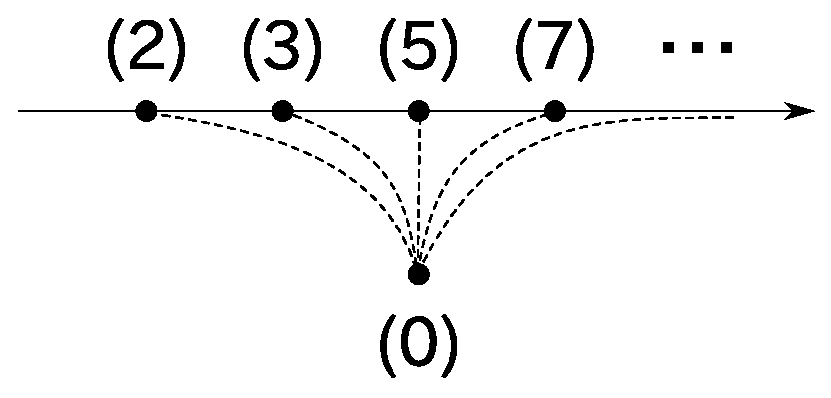
\includegraphics[width=5cm]{./images/SpecZ.eps}
    \end{center}
    \end{figure}

    $\Spec \Z$の開集合は,$\emptyset, \Spec \Z$,$\Spec \Z$から有限個の点を除いたもの.
    (TODO)

\section{$\Spec \{0\}$ is the Initial Object in $\Sch$.} %% Ex2.6 
    零環$\{0\}$はただひとつのイデアル(したがって素イデアル)$(0)$を持つから,$\Spec \{0\}$は1点集合.
    零環から別の環への準同型写像は$0 \mapsto 0$なるものしか無い.
    schemeの間の射は環の間の準同型から作られるものしかないから(Prop2.3c),
    $\Spec \{0\}$から別のschemeへの射は$0 \mapsto 0$から得られるものしか無い.
    よって$\Spec \{0\}$はinitial object.

\section{ } %% Ex2.7 

\section{ } %% Ex2.8 

\section{ } %% Ex2.9 

\section{ } %% Ex2.10 

\section{ } %% Ex2.11 

\section{ } %% Ex2.12 

\section{ } %% Ex2.13 

\section{ } %% Ex2.14 

\section{ } %% Ex2.15 

\section{ } %% Ex2.16 

\section{ } %% Ex2.17 

\section{ } %% Ex2.18 

\section{ } %% Ex2.19 


\end{document}
